% article document class appropriate for small (<100 pages) documents
\documentclass[draft, english, a4paper]{article}

% Packages provide additional functionality
%\usepackage{url}
\usepackage{fixme}
%\usepackage{lmodern}
\usepackage[final]{graphicx}%Force the graphics package to final, to force image inclusion
\graphicspath{{eps/}{images/}} %Set images/figures search path (relative to top latex file)
\usepackage[utf8]{inputenc}
\usepackage[left=3cm,top=4cm,right=3cm]{geometry}
\usepackage{listings}
\usepackage[dvips,
            colorlinks=false,
            pdfduplex=DuplexFlipLongEdge,
            pdfborder={0 0 0},
            pdftitle={Playing with LEGO},
            pdfauthor={Mikael Moghadam, Kenni Peter Isaksen, Morten S. Laursen,
                Robot Technology,
                SDU,
                Odense,
                Danmark},
            pdfsubject={Introduction to Artificial Intelligence},
            pdfkeywords={LEGO, Sokoban, line follow},
            plainpages=false,
            final]{hyperref}

\title{Playing with LEGO}
\author{Mikael Moghadam, Kenni Peter Isaksen, Morten S. Laursen}

\begin{document}

\maketitle % reads info from \title and \author above


% where BibTeX should read the bibliography records from and what
% style of bibliography it should generate
%\bibliographystyle{plain}
%\bibliography{}
\section{Introduction}
\newpage
\tableofcontents
\newpage
\section{Architecture}
	\subsection{Division of responsibilities}
	The architecture of the system is composed of two separate systems, a planner and a physical robot.
The planner runs on a PC and is responsible of creating a file with the actual plan, for solving the task at hand. The planner takes a map as input and uses a search-algorithm to find the right path to the goal in a search tree. When the right path is found a file with the robot-navigation-commands is created.

The robot-navigation-command-file contains a string of commands. These commands are up, down, right, left and turn around, they are represented as 'u', 'd', 'r', 'l' and 'a' in the file.

The file created by the planner is used by the robot to correctly navigate the map as fast as possible. The robots task is to move from one field on the map to another as fast as possible and at the same time follow the line.  The robot itself does not perform any path-finding, but only navigates the map using the commands from the file created by the planner. 


\section{Robot description}
        The purpose of this prototype is to perform the assignment as described by
        the planner. In order to accomplish this task a robot 
        has been created. The robot is created using the LEGO NXT platform. 
        \begin{figure}[htp]
            \centering
    	    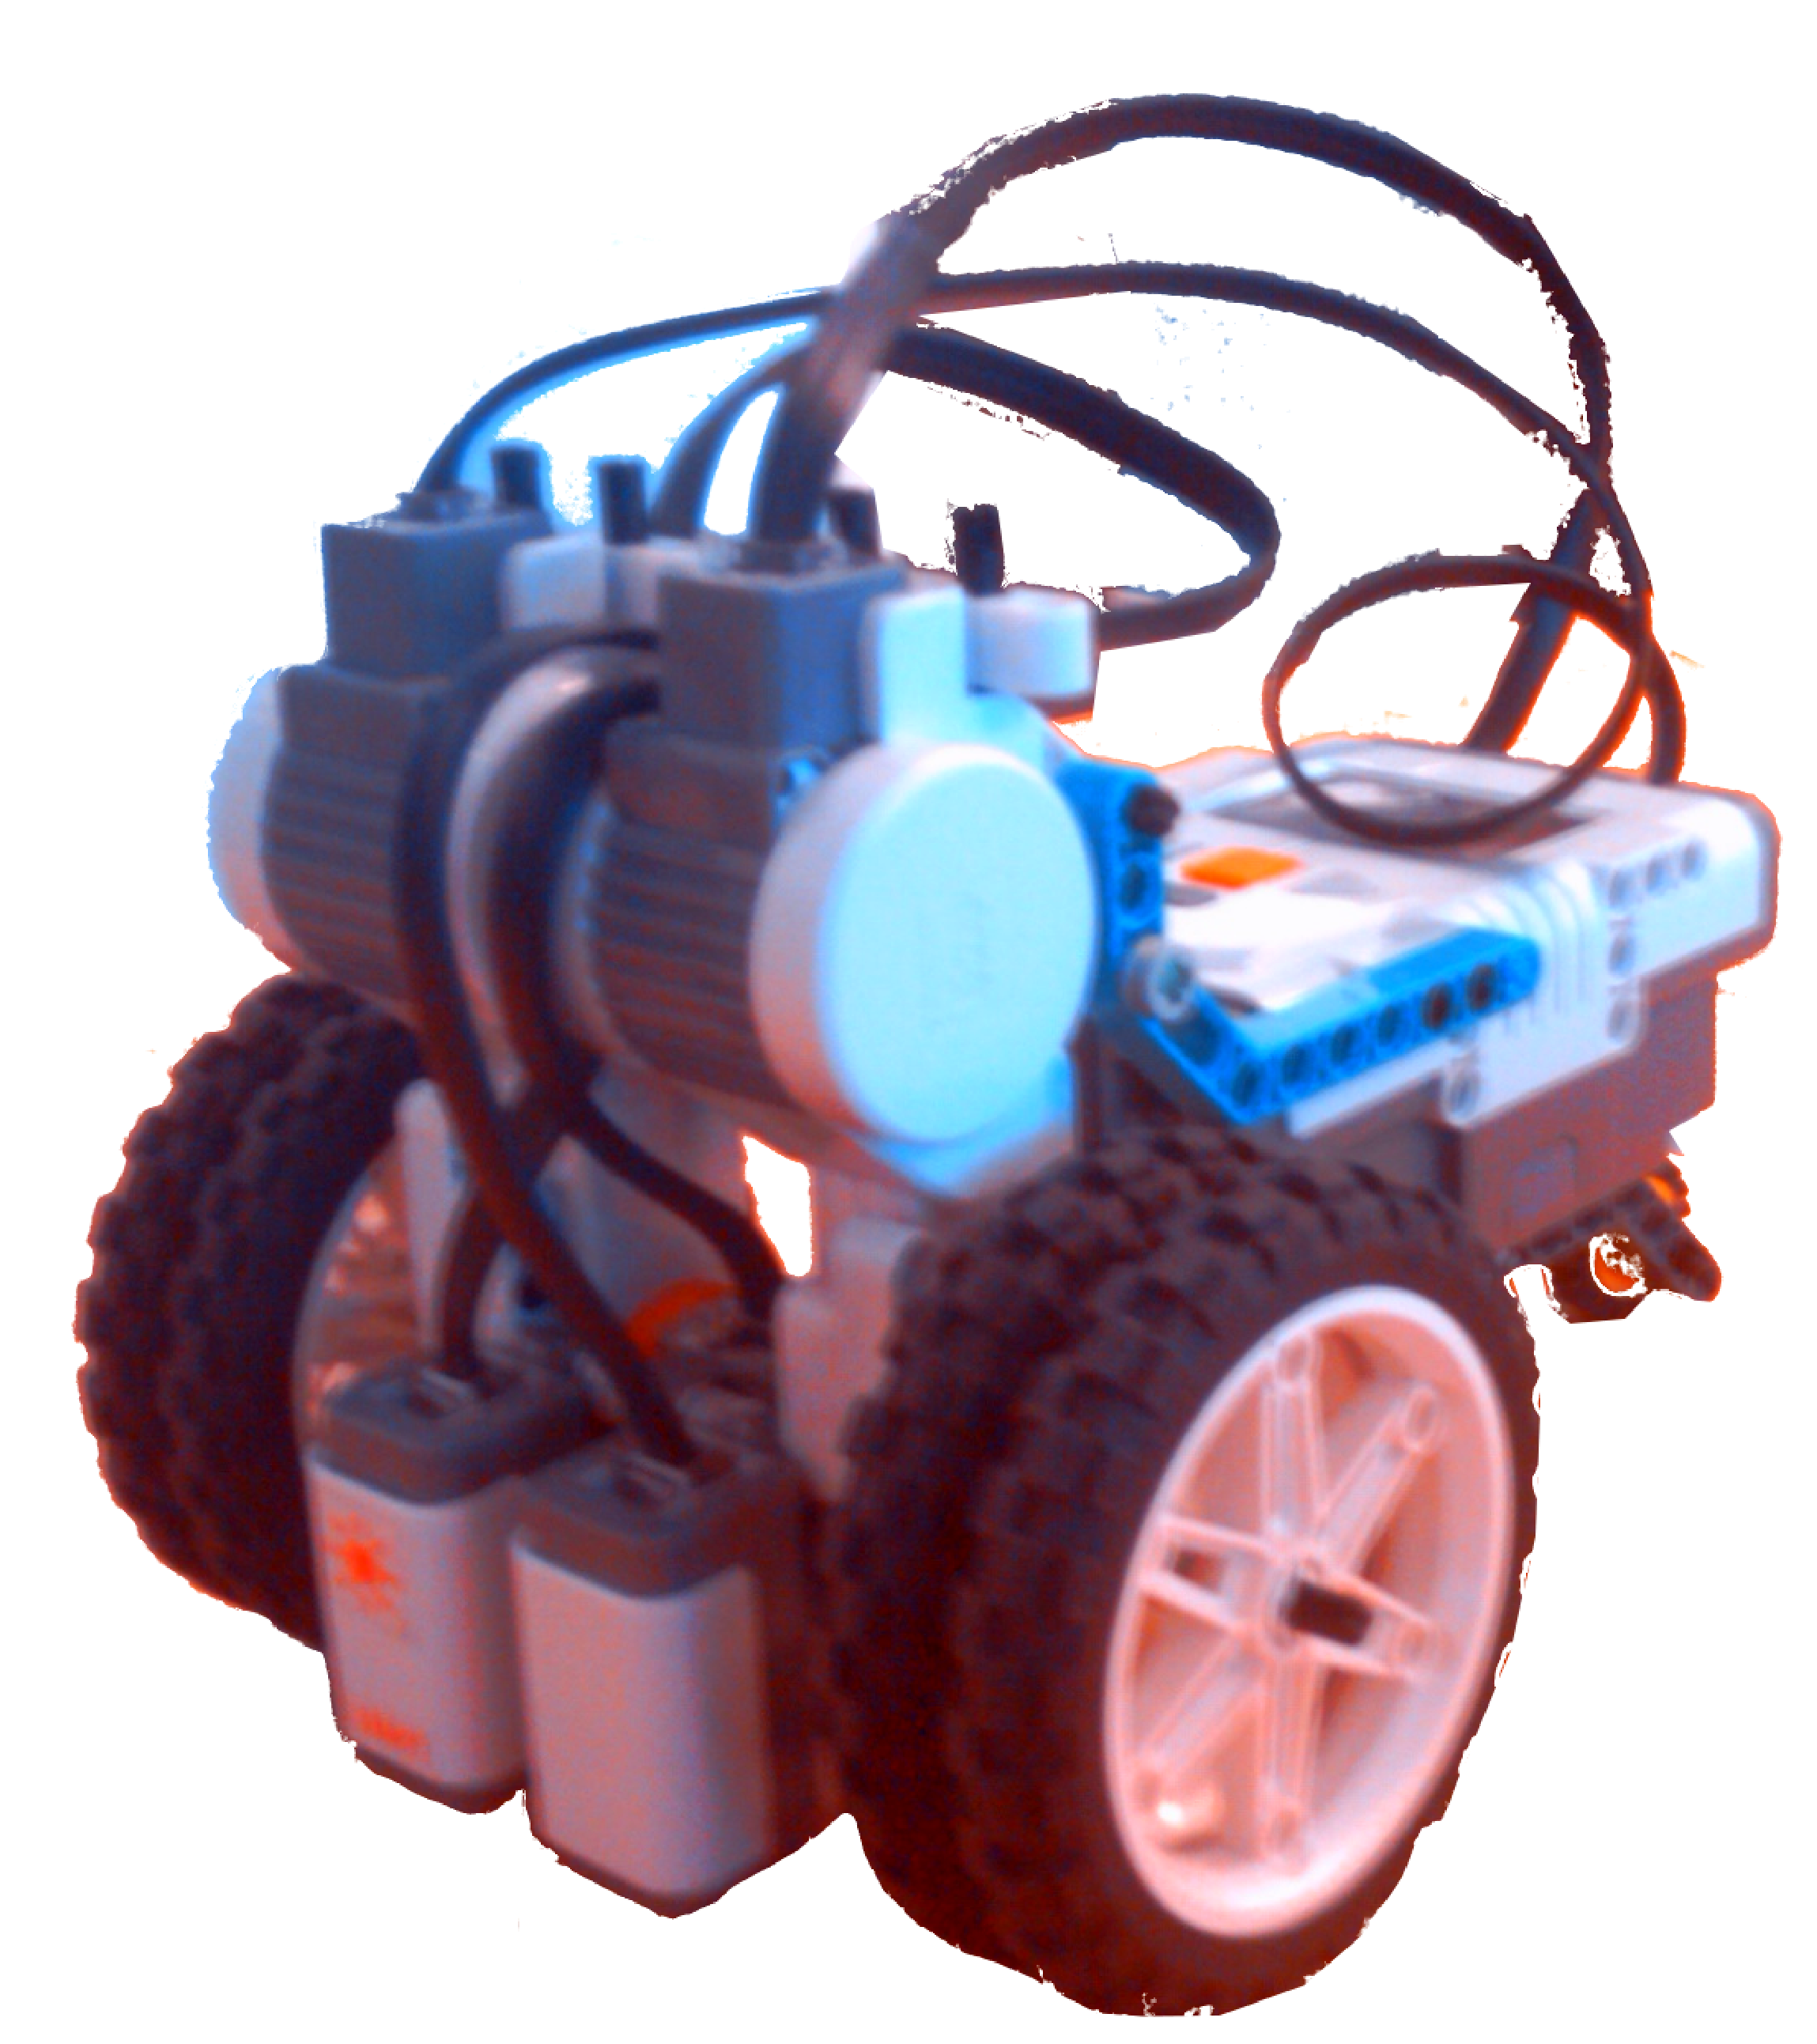
\includegraphics[scale=0.1]{robot}
	        \caption{Picture of the robot in it's current state}\label{fig:robotPic}
        \end{figure} 
	\subsection{Physical Construction} %Morten  
	    \label{robot:physicalContruction}
	    The robot is constructed using two motors which applies force to
	    each of their front wheels, this allows the robot to steer using skid steering.
	    As close as possible to the center of rotation during turns, three light
	    reflectance sensors is placed as illustrated in figure \ref{fig:lightSensorPlacement}
	    \begin{figure}[htp]
            \centering
    	    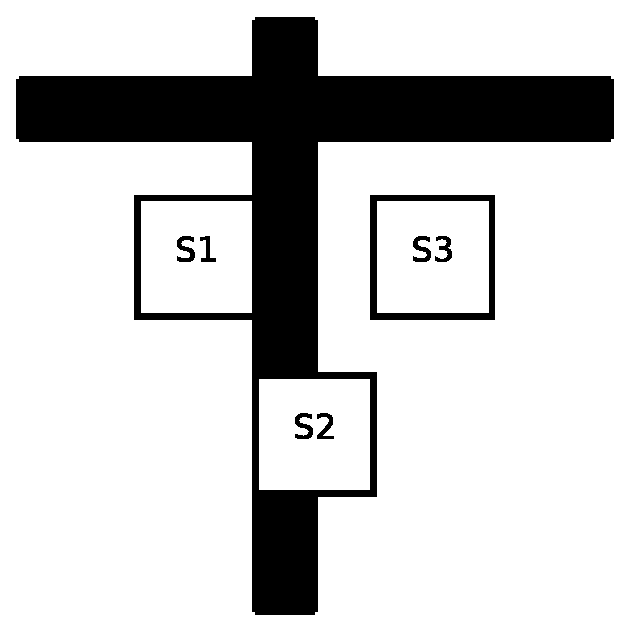
\includegraphics[scale=0.45]{lightSensorPlacement}
	        \caption{Illustration of light sensor placement, with the sensors mentioned S1-S3}\label{fig:lightSensorPlacement}
        \end{figure}
	    This allows the robot to detect either side of the line and thereby to
	    follow it, furthermore it allows the robot to detect when crossing a 
	    line.
	      
	\subsection{Robot architecture}
	    The Software architecture for the robot is devided into layers
	    this is performed to give an abstraction
	    of each layer with as little complexity as possible. The architecture
	    is best illustrated by the block diagram illustrated in figure \ref{fig:robotBlockDiagram}.
	    \begin{figure}[htp]
            \centering
    	    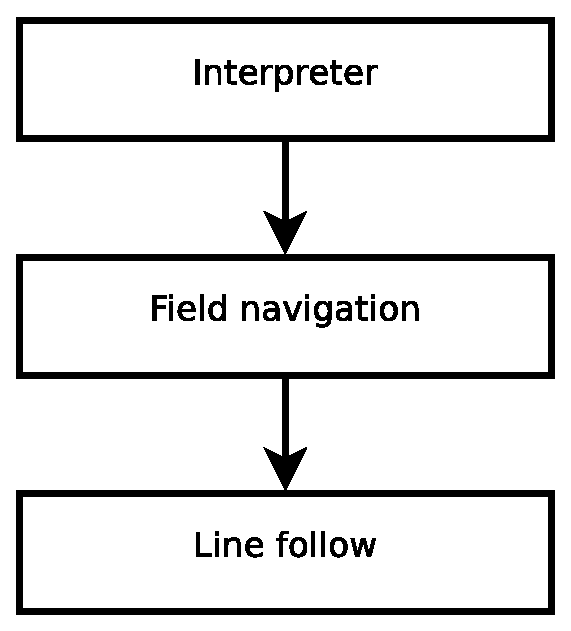
\includegraphics[scale=0.45]{robotBlockdiagram}
	        \caption{Block diagram of LEGO robot}\label{fig:robotBlockDiagram}
        \end{figure}
		%General introduction
		%block diagram
		\subsubsection{Interpreter} %Morten
		    The interpreter has to receive and interpret data from the routeplanner
		    and carry out that route using the field navigation block.\\
		    \\
		    The flow chart for the interpreter can therefore be described in the
		    following way
		    \begin{enumerate}
		    \item Receive/fetch command from routeplanner
		    \item perform command using field navigation
		    \item if more commands in cue goto 1, else exit
		    \end{enumerate}
		    Currently two options is under consideration for the interface between
		    the interpreter and the routeplanner, one is a simple file composed
		    of direction commands as delivered with the Sokoban example game.
		    The other option is to stream the commands using bluetooth, it is
		    anticipated that this would allow for easier debugging, and because
		    of existing libraries for bluetooth it should not cause much if any overhead.\\
		    \\
		    \fixme{For discussion: Should the interpreter or the routeplanner be responsible of
		    tomato can attack directions?}
%			What is the responsibility of this block
%			Block interface
%			Block design / bird perspective flow chart 
%			Block test
		\subsubsection{Field navigation} %Morten
		    The field navigation should navigate between field intersections
		    as illustrated on figure \ref{fig:robotFieldNavigation}.
		    This task should be accomplished using the line following block\\
		    \begin{figure}[htp]
                \centering
    	        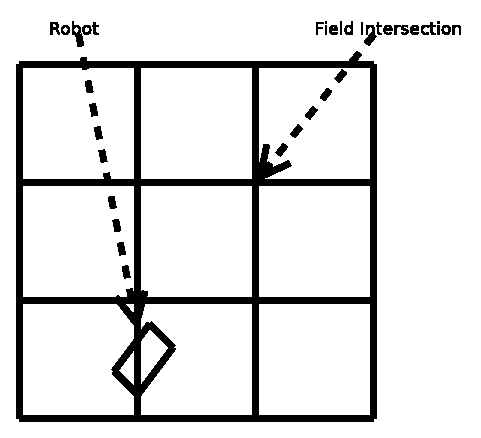
\includegraphics[scale=0.45]{robotFieldNavigation}
	            \caption{Illustration of playing field}\label{fig:robotFieldNavigation}
            \end{figure}
		    \\
		    As described in section \ref{robot:physicalContruction} the light
		    sensors is placed so that when following lines, only one sensor should
		    be active at a time, however when crossing a line both the left and the
		    right sensor should become active. This allows the robot to detect
		    crossing lines.\\
		    \\
		    When crossing a line the robot should first back up, so that the sensors
		    is placed over the crossing line, then rotate in the commanded direction
		    until a new line activates both sensors, then move one field
		    forward.
		    \fixme{Another option here is using the encoders
		    in reality we might test both and see which one performs best}
%			What is the responsibility of this block
%			Block interface
%			Block design / bird perspective flow chart 
%			Block test
		\subsubsection{Line follow} %Morten
		    The line following block has the responsibility of keeping the robot
		    constantly on the line using the sensors to allow for precise navigation.\\
		    \\
		    On figure \ref{fig:sensor_measurements} a plot of what the sensors
		    measures when driving on a line has been created. It is clear when
		    looking at the plot that the signal does not contain a lot of higher
		    frequency components and will therefore not gain much from being filtered,
		    except less phasemargin in the control system. These data was measured
		    doing a evaluation of a proportional feedback control system.
		    \\
		    \begin{figure}[htp]
                \centering
    	        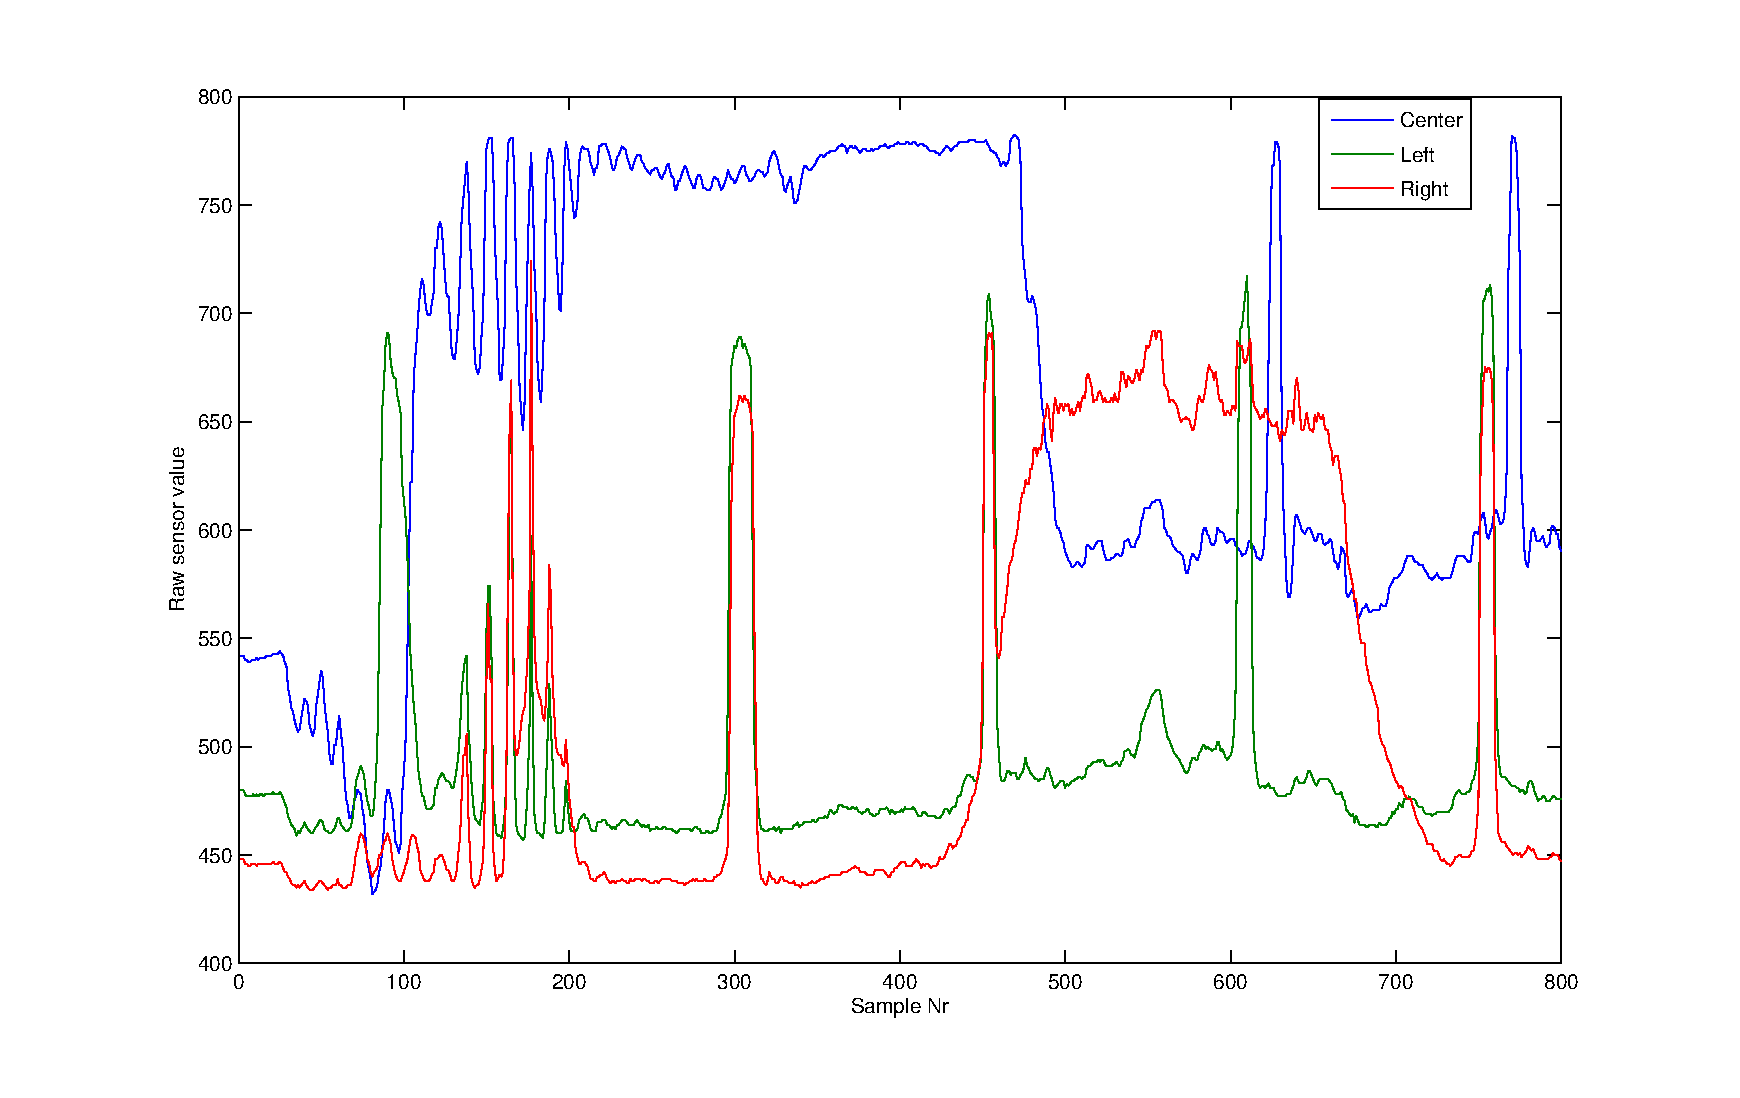
\includegraphics[scale=0.45]{sensor_measurements}
	            \caption{Raw samples of sensor measurements}\label{fig:sensor_measurements}
            \end{figure}
            \\
            \paragraph{Statemachine based}
            For making the control loop two different implementations has been
            tested, one using a simple state machine based solution, where the
            state machine tries to assess the position of the line as either left of the
            vehicle, centered below the vehicle or right of the vehicle and from
            this assessment tries to correct.\\
            \\
            \paragraph{PD-feedback based}
            Another option which has been tested is making a simple PD control loop
            using the light sensors, as the sensors are not entirely binary,
            but has a slight transition as more and more of the sensed area becomes
            line, it increases, a correction based on these small increases can 
            be seen as the oscillation between sample 100 - 200 on figure \ref{fig:sensor_measurements}
            Whereas the state machine based approach does not start correcting before reaching a threshold value.\\
            \\
            Having implemented both solutions on the vehicle the control loop based
            solution was chosen as it had the best performance.
		    %More detailed problem description with sensor position drawing
		    %measurement data examples.
		    %From there show proposed solutions
		    %Explain which one was chosen for which reasons, show flow diagrams
		    %of these two algorithms 
		    %Show incoming and output data from this block and the module test
%		    What is the responsibility of this block
%			Block interface
%			Block design / bird perspective flow chart 
%			Block test
	\subsection{Conclusion} %Morten
	    \fixme{Let us write this when the vehicle is done}
\section{Planner description}
    \subsection{Problem discussion, in the Sokoban domain}
Sokoban is a game originating from Japan. The essence of the game is to push jewels around in a room containing obstacles, in a manner that will enable the player to place all the jewels on so called goals in the room. See figure \ref{fig:sokohero} for a screenshot of a sokoban game.
Sokoban is an interesting game to study in the domain of Artificial Intelligence, because it presents a so called NP-complete problem, meaning in this case that it is often fairly easy for humans to solve such puzzles in a manner of minutes, but very difficult to develop an efficient algorithm able to do the same. This is due to the fact that NP-complete problems spawn huge search trees and branch factors.

\subsubsection{The rules of the game}
The rules of the game are simple. The game is best described as consisting of squares, each having an (x, y) coordinate. A game consists of the following squares:
\begin{itemize}
\item One 'Man' square, representing the player. The 'Man' square can move around.
\item One or more 'Jewel' squares representing objects that have to be pushed onto 'Goal' squares by the player.
\item One or more 'Goal' squares. There are always the same amount of 'goal' squares as 'Jewel' squares.
\item One or more 'Wall' representing impenetrable boundaries which can not be passed by neither 'Man' nor 'Jewel' squares.
\item One or more 'Empty' squares representing space where the player/'Man' square is able to move. 
\end{itemize}

\begin{figure}[ht]
\centering
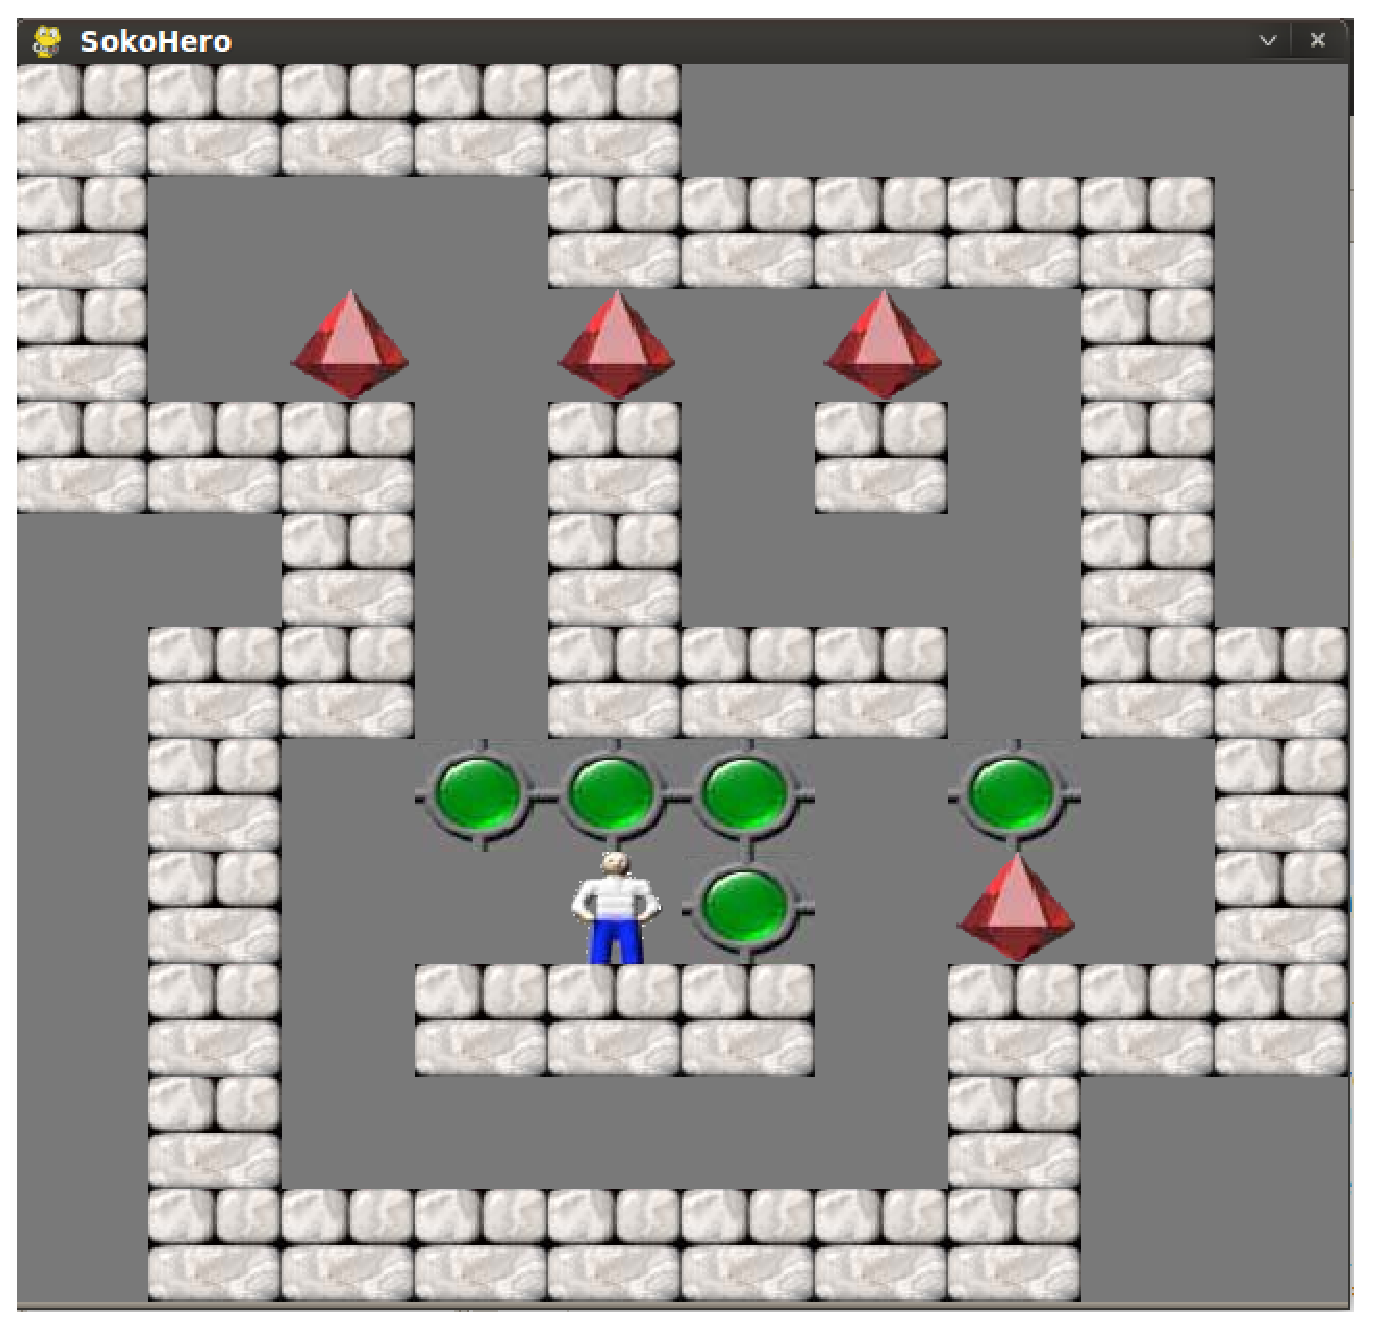
\includegraphics[scale=0.25]{images/sokohero.eps}
\caption{A screenshot of a sokoban game}
\label{fig:sokohero}
\end{figure}


As stated previously the purpose of the game is for the player to push 'Jewel' squares onto 'Goal' squares. That the player is only able to push jewels signifies that if a jewel is at position (x, y), and the player is at position (x - 1, y) then the player will be able to move the jewel to position (x + 1, y) if (x + 1, y) is occupied by an 'Empty' or a 'Goal' square. The same logic applies for other directions.
 
\subsubsection{Challenges faced when solving Sokoban algorithmically}
Given the fact that the player can on average move up, down, left and right, we see that the problem presents a so called branching factor of 4. If an algorithm is able to solve the puzzle in 100 moves, the complexity becomes 4$^{100}$ . 
This enormous complexity, illustrates the need for some sort of heuristics or pruning of the search tree, if the problem is to be solved in an acceptable time frame.
Deadlocks are one of the main challenges faced when trying to solve the Sokoban puzzle. A deadlock is best described as a situation where a jewel is pushed into a position that eliminates the possibility of solving the puzzle, for instance pushing a jewel into a corner. 

\subsubsection{Algorithmic approach}
The general approach taken to solve the sokoban problem, is creating a search tree where every node in the tree is a state of the game. The goal is then to traverse the tree to find the state where all of the coordinates of the jewels match the coordinates of all the goals.\\
The general algorithmic search can described as:

\begin{lstlisting}[language=Ruby, frame=single, basicstyle=\tiny, caption={Deadlock detection pseudo code}, label={code:sokoalgo}]
if not problem solved:
	get next state in search tree
	if state not goal state:
	  for each jewel in state do:
	    for every direction in which jewel can move one square do:
		  if resulting state is valid and not duplicate of a previous state:
		   if robot can get to the position to push the jewel in the desired direction:
             create new state				
			 move jewel to new position
			 move robot to previous jewel position
			 calculate state score
			 add state to search tree	
\end{lstlisting}

As can be seen from the pseudo code, the problem solving can logically be divided into two separate subproblems, the first one being the movement of the jewels, henceforth known as the jewel problem, and the second being the path finding from the robot to the jewel that has to be moved, henceforth known as the path finding problem. 
The search approach best suited for the solving of these two distinct areas might not be the same, and therefore each subproblem is considered separately, and the solution implemented will treat the subproblems as two seperate search trees. 
It is important to note that the optimal solutions is wanted in terms of minimum number of robot/man movements. This is as mentioned due to the fact that the competition is on time, and the assumption therefore is that the less squares that the robot has to traverse, the less time it will take to solve the puzzle.
	\subsection{Discussion of search algorithms} %Mikael
		\subsubsection*{The following algorithms have been considered to solve the jewel problem}
As mentioned the two things that can potentially hope to minimize the search time needed to solve a sokoban problem, namely a 'good' heuristic search and search tree pruning. The search algorithm, and therefore by extension also the heuristic function, is concerned with the 'get next state in search tree' part of the algorithm in listing \ref{code:sokoalgo}, and pruning is concerned with the 'is state valid' part.

\subsubsection*{A*}
This was the first algorithm considered using for the problem, because it is both optimal, complete and fast if a good heuristic function is used.
It has however proven fairly difficult to find a 'good' admissible heuristic for the jewel problem. One of the only possibilities that have come to mind is the sum of each jewels manhatten distance to it's closest goal. This heuristic would be admissible, since the closest distance from a jewel to a goal would naturally be the minimum amount of moves needed to move the jewel in order to solve the problem. It is our assessment that this heuristic unfortunately can not be characterized as a very good one, since the sum of smallest distances between jewels and goals, is by no means an estimate of the number of moves left to solve the problem, due to the intrinsic complexity of most sokoban problems (jewels getting in the way of other jewels, jewels being blocked by walls etc.). In other words, a good A* heuristic should guide the search down the branch of the search tree most likely to contain an acceptable solution, thereby minimizing the nodes/states that would have to be traversed in order to get to a solution. The considered heuristic would not necessarily be able to do so.
The cost that would be used in this implementation, would be the total number of moves the robot/man would have to take to move the jewel to the desired position plus the robot moves taken to get from the initial state (root state) to the current state.

\subsubsection*{Greedy search}
By disregarding the Heuristic function from the A* search, and instead using the cost of robot movements as the heuristic, we would in effect get a greedy search. We would use a so called closed list, to avoid loops, thereby attaining completeness. The downside of this algorithm however is that it is not optimal, which is a requirement if we are to get a solution with the minimum required number of robot movements.

\subsubsection*{Breadth first search}
The breadth first search algorithm is inherently slow for complex problems, but is however optimal in so called unit-step cases (the cost from one state to the next is always the same), which speaks greatly in favour of this algorithm in this case. However for this to work it is important to remember that the unit-step requirements necessitates an implementation where each robot movement spawns a new state, as opposed to just spawning a new state for each jewel movement, so that the depth of the solution in the tree will correspond with the number of movements performed by the robot. The use of this algorithm therefore requires that the two subproblems be solved as one. This will, among other things, increase the amount of memory needed by the algorithm. 

\subsubsection*{Uniform cost search}
A variation on the breadth first search and greedy search exists, where the next node visited is the one with the least total cost from the root node (the same cost as used in the A* algorithm), as opposed to the greedy search where the next state visited is the one with the least cost from the current node, which was the cause of the non optimality of the greedy search. This is therefore both a complete and optimal algorithm in terms of minimum robot movements, when using the robot movements as cost. Furthermore it does not require, as the breadth first search, that the sokoban problem not be solved as two subproblems.

\subsubsection*{Search tree pruning}
Since a good heuristic function has not been found for the search algorithm, the time complexity of the solver will presumably be high, unless the search tree can be pruned significantly. Fortunately the sokoban problem is one where a large amount of pruning is possible in terms of deadlock detection. 

\begin{figure}[ht]
\centering
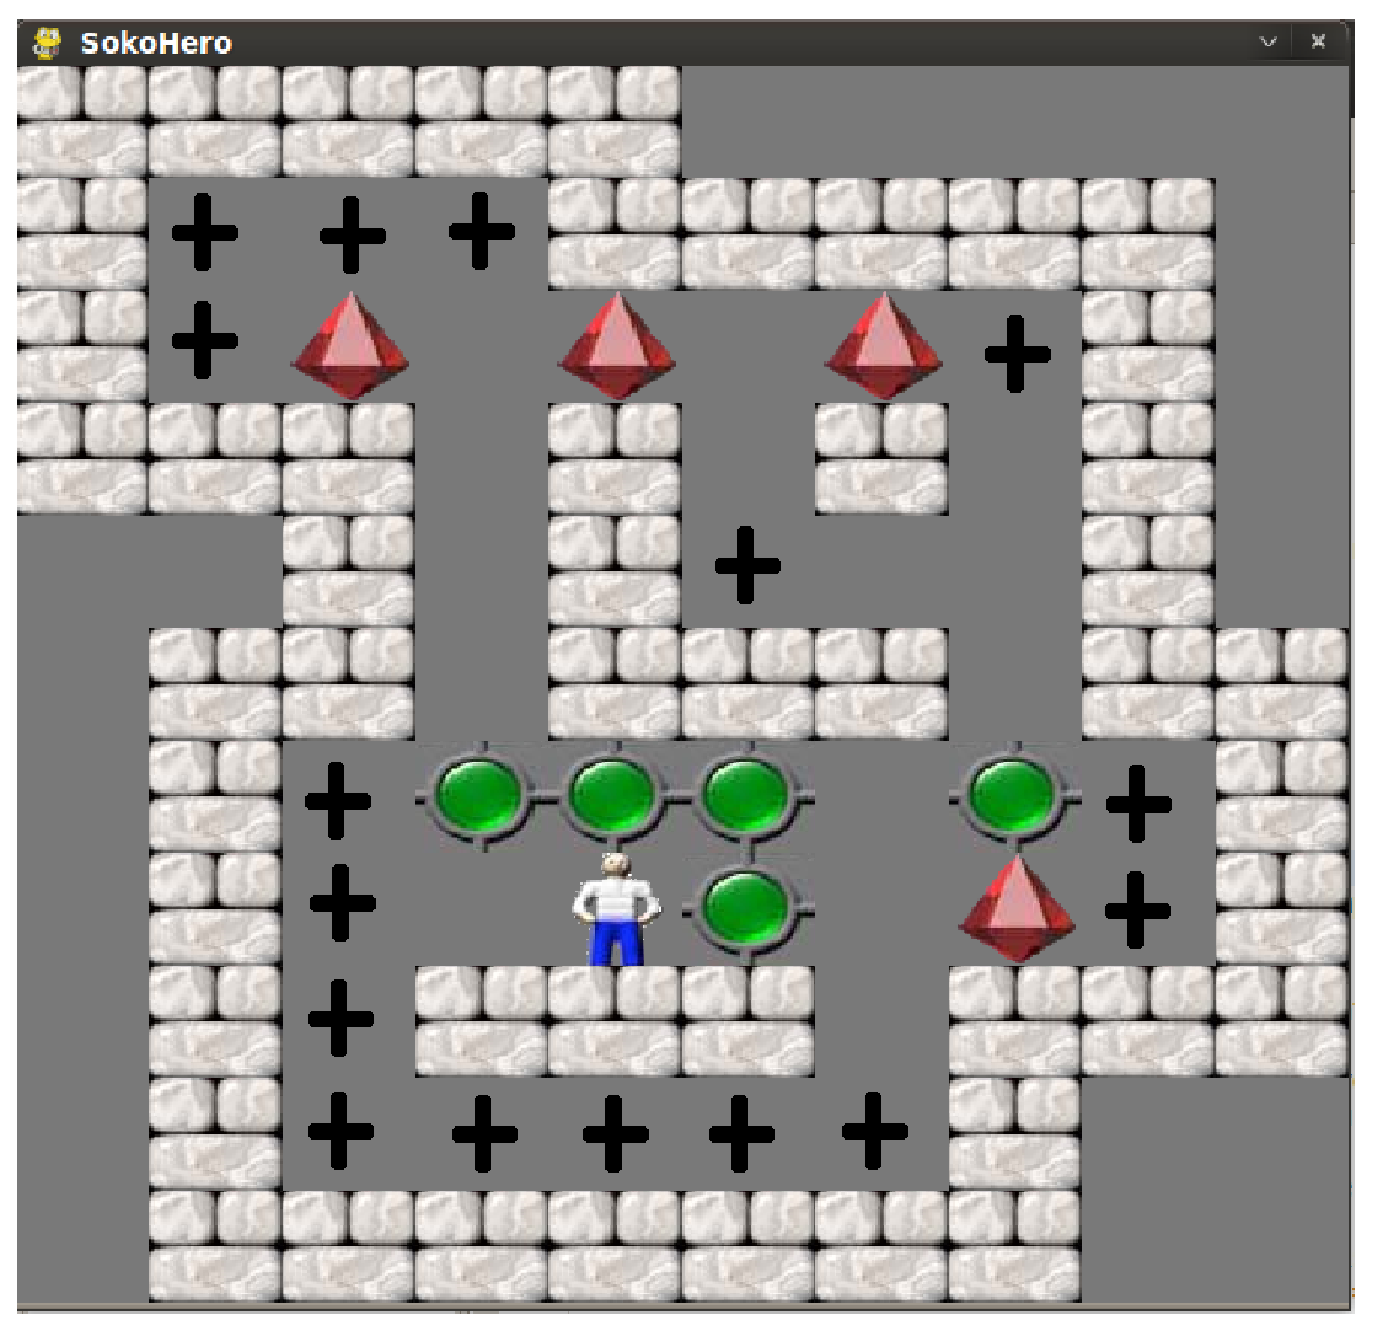
\includegraphics[scale=0.25]{images/sokohero_deadlocks.eps}
\caption{A screenshot of a sokoban game with deadlock zones marked with '+'}
\label{fig:sokoherodeadlocks}
\end{figure}

Figure \ref{fig:sokoherodeadlocks} shows all the zones where the placement of a jewel would result in an unsolvable problem, meaning that the state and all states spawned from that one are useless, and would only potentially waste the time of the solver if it would have to visit them.
\\
The following deadlock detection algorithm is devised, where return true symbolises that the state has a deadlock:

\begin{lstlisting}[language=Ruby, frame=single, basicstyle=\scriptsize, caption={Deadlock detection pseudo code}, label={code:deaddetect}]
For each jewel do:
  if jewel in corner:
    return true
  if jewel against vertical wall:
    for each square above jewel:
      if square is goal:
        return false
      if square on the obstructed side of jewel is empty or goal or jewel:
        return false
    for each square below jewel:
      if square is goal:
        return false
      if square on the obstructed side of jewel is empty or goal or jewel:
        return false
  if jewel against horizontal wall:
    for each square to the right of jewel:
      if square is goal:
        return false
      if square on the obstructed side of jewel is empty or goal or jewel:
        return false
    for each square to the left of jewel:
      if square is goal:
        return false
      if square on the obstructed side of jewel is empty or goal or jewel:
        return false
  return true
\end{lstlisting}

This deadlock detection algorithm could be improved further by checking for deadlocks due to one jewel obstructing another in a irreversible way. Due to the deadline of the project however, it has not been possible to include this feature.

\subsubsection*{The following algorithms have been considered to solve the path finding problem}
\subsubsection*{A*}
This algorithm is very often used as path finding algorithms in games, because good heuristic functions are relatively easy to find when confronted with such problems. Often the manhatten distance to the goal is sufficient enough to give very fast searches compared to depth- or breadth first. Therefore we do not consider any other searches for the path finding problem.

\subsection{Choosing the search algorithm}
Naturally the A* algorithm will be used to solve the path finding problem. The choice of search algorithm for the jewel problem would have fallen on the Uniform Cost Search algorithm, because it gives an optimal solution in terms of robot movements which is of most importance, since the time to solve the problem is irrelevant because the specific problem as mentioned will be given a week in advance. We will however, out of pure academical interest, implement all of the considered algorithms for the jewel problem, in order to compare their performances. 

	\subsection{Implementation}
	\subsection{Choice of programming language}
The first language considered for implementing the solver, was Python. Python however turned out to be very slow for this type of problem, in particular when using a debugger. We therefore turned to java, because java still provides a significant programming abstraction compared to C or C++, allowing us to focus more on the algorithms than on memory allocation and deallocation. Furthermore java has a standard library that is more mature and easier to use than the standard template library of C++. 



	\subsection{Performance evaluation}
	For each search algorithm, three consecutive runs have been performed with each search algorithm, and the data from the best run chosen.\\

\begin{table}[h!]
	\centering
	\begin{tabular}{| l | c | c | c | c | }
		\hline
			Search algorithm	& States traversed & Memory used [MB] & Robot moves & Time taken [s]\\ \hline
	    	Uniform Cost & 18968 			& 39 		 & 142 	& 202\\\hline
		    Breadth first (Non unit-step)	& 19761 			& 40 		 & 162 	& 218\\\hline
		    A*		& 18788 			& 39 		 & 142 	& 189 \\\hline
	    	Greedy 		& 18215 			& 48 		 & 212 	& 179 \\
		\hline
	\end{tabular}
	\label{tbl:searchresults}
	\caption{Results from the different search algorithms.}
\end{table}
\\
Another search has been performed with the tree pruning algorithm disables (No removal of deadlock states), to see how big and effect the pruning has on the performance of the solver. The search algorithm used is A*, because it outperformed the other search algorithms.\\
\begin{table}[h!]
	\centering
	\begin{tabular}{| l | c | c | c | c | }
		\hline
			Search algorithm	& States traversed & Memory used [MB] & Robot moves & Time taken [s]\\ \hline
		    A*		& 148097 			& 318 		 & 142 	& 12223 \\
		\hline
	\end{tabular}
	\label{tbl:searchresultsnoprun}
	\caption{Results from the different search algorithms, when search tree pruning is disabled.}
\end{table}


\subsection{Planner conclusion}
As can bee seen from the Uniform Cost search in table \ref{tbl:searchresults}, the optimal solution contains 142 robot movements (102 if the solver did not take into account the number of moves that the robot must perform in reality). As predicted the breadth first and greedy searches do not find the optimal solution, and would therefore not be applicable to use for this particular project, even though greedy search outperforms the other searches in terms of speed. As it turns out the A* search outperforms the Uniform Cost Search in number of states traversed and time taken, which was not all that unexpected. It can therefore be concluded that the sum of the manhatten distances between the each jewel and its closest goal, is a heuristic that will yield an optimized search. It can furthermore be seen from table \ref{tbl:searchresultsnoprun}, as expected that the effects of pruning far outweigh the gains that one particular search algorithm provides over another in terms of time taken to find solution, the states traversed and the memory used.

\section{Conclusion}
\section{Discussion}
\bibliographystyle{plain}
\bibliography{bibtex_refs.bib}
\appendix
\end{document}

